% =====================================================================
%  ACoT-UAV-Track — paper first draft
%  Generated from acot_note/ (design doc, ACoT-VLA reading, dataset card,
%  training plan) and positioning-analysis.md.
%
%  STATUS: FIRST DRAFT / SCAFFOLD.
%  - The model has NOT been trained yet (training is the next stage in the
%    project notes). Therefore every quantitative RESULT is a visible
%    placeholder rendered by \ph{...} (red). Do not submit until these are
%    replaced with measured numbers.
%  - Benchmark/dataset numbers ARE real (from acot_note/dataset-card.md).
%  - Every citation must be verified against the source before submission;
%    see references.bib header and README.md.
%
%  Single-column article for portability. Swap \documentclass for a venue
%  style (CoRL/ICRA/NeurIPS) when the target is chosen.
% =====================================================================
\documentclass[11pt]{article}

\usepackage[utf8]{inputenc}
\usepackage[T1]{fontenc}
\usepackage[margin=1in]{geometry}
\usepackage{graphicx}
\usepackage{amsmath,amssymb}
\usepackage{booktabs}
\usepackage{multirow}
\usepackage{xcolor}
\usepackage{colortbl}
\usepackage[numbers,sort&compress]{natbib}
\usepackage[colorlinks=true,linkcolor=black,citecolor=blue,urlcolor=blue]{hyperref}
\usepackage{enumitem}
\usepackage{caption}
\captionsetup{font=small,labelfont=bf}

% --- Placeholder for results that do NOT yet exist (rendered red). --------
\newcommand{\ph}[1]{{\color{red}\textbf{[#1]}}}
% --- Term the author should verify (rendered orange). --------------------
\newcommand{\chk}[1]{{\color{orange}#1}}

% --- Locked terminology (single canonical form; see README ledger). ------
\newcommand{\sys}{ACoT-UAV-Track}
\newcommand{\ear}{EAR}
\newcommand{\iar}{IAR}
\newcommand{\agp}{AGP}
\newcommand{\zex}{Z^{\mathrm{ex}}}
\newcommand{\zim}{Z^{\mathrm{im}}}

\title{\textbf{\sys{}: Action-Space Chain-of-Thought for\\
Language-Conditioned Aerial Vehicle Tracking\\
under Similar-Distractor Disambiguation}}

\author{%
Anonymous Author(s)\thanks{Author list, affiliations, and funding to be
completed by the authors.}\\
\texttt{hque@nvidia.com}
}
\date{}

\begin{document}
\maketitle

% =====================================================================
\begin{abstract}
% Task -> gap -> what the system is (credited transfer) -> what is new
% (the benchmark / task intersection) -> evidence plan (placeholders).
Embodied visual tracking asks an agent to keep a moving target in view by
acting, not merely by perceiving. In the air, this couples a slow decision
(\emph{where is the target going}) with a fast one (\emph{keep it centred}),
and language makes it harder still: the agent must fly to follow \emph{one}
car named in a sentence while several visually similar vehicles drive nearby.
Prior work solves neighbouring pieces of this problem---aerial
language-conditioned tracking without distractor disambiguation, ground
tracking that disambiguates similar distractors, or passive UAV
referring perception that never controls the aircraft---but no published
system closes the loop on all four axes at once: active flight, a
language-specified target vehicle, disambiguation among visually similar
distractor vehicles, and closed-loop embodied control. We present
\sys{}, a vision-language-action (VLA) model for this intersection. Its
reasoning core---an Explicit Action Reasoner (\ear{}) that denoises coarse
3D interception waypoints, an Implicit Action Reasoner (\iar{}) that reads
per-layer priors from a frozen vision-language backbone, and an
Action-Guided Prediction (\agp{}) head that fuses both into a
flow-matching action expert---is transferred from ACoT-VLA
\citep{acotvla}; our contribution is to adapt this action-space
chain-of-thought to the aerial vehicle-disambiguation setting and to build
a CARLA benchmark whose scene design and counterfactual-language protocol
make language \emph{load-bearing} rather than a decorative input. We further
replace discrete track/search/recover mode switching with a single
continuous, differentiable \texttt{search\_mode} dimension. We describe a
staged training pipeline (backbone grounding probe, waypoint warm-up,
end-to-end curriculum, optional closed-loop RL) and an evaluation protocol
built around mis-follow rate, occlusion-recovery rate, and held-out-town
generalisation, with language-necessity ablations at its centre.
% NOTE: the model is not yet trained; all quantitative results below are
% placeholders to be filled after Stage 1--2 training completes.
On the proposed benchmark we expect \sys{} to \ph{result: SR / mis-follow
gain vs.\ UAV-Track VLA and appearance-only baseline}, with the
language-necessity ablation showing \ph{result: mis-follow rise when
language is removed}. We release the benchmark, data-generation pipeline,
and evaluation code to support this under-served task.
\end{abstract}

% =====================================================================
\section{Introduction}
\label{sec:intro}

% Para 1: task + application (Version 3: general task -> specific setting)
Embodied visual tracking---an agent that moves to keep a designated target
within its field of view---underpins aerial applications such as cinematic
follow-shots, search-and-follow of a suspect vehicle, wildlife and convoy
monitoring, and infrastructure escort. Unlike passive video object
tracking, the agent's own actions determine what it will see next: a poor
control decision loses the target, and no amount of downstream perception
recovers it. This paper studies a specific and, we argue, under-served
setting of this problem: a single unmanned aerial vehicle (UAV) that must
fly to follow \emph{one} target vehicle, specified only by a natural-language
description, while several \emph{visually similar} vehicles drive in the
same scene.

% Para 2: previous methods -> the technical/setting gap (this is where the
% contribution lives). Cut precisely against the closest competitors.
Three lines of recent work each solve part of this setting but leave the
combination open. \emph{Aerial VLA tracking} produces closed-loop flight
from language, but its scenes are not built to force disambiguation among
look-alike targets: UAV-Track VLA \citep{uavtrackvla} flies to track a
language-named pedestrian or vehicle in CARLA with an explicit
3D-localisation head, yet does not emphasise similar-distractor
disambiguation. \emph{Distractor-robust embodied tracking} disambiguates
targets from confusers, but on the ground and usually without language:
TrackVLA++ \citep{trackvlapp} equips a quadruped tracker with a
polar-coordinate action chain-of-thought and an explicit target-identity
memory, and DeTrack \citep{detrack} performs closed-loop UAV tracking with
moving distractors and obstacle avoidance but without a language channel.
\emph{UAV language referring} names a target among similar vehicles, but
only passively: UAVNLT \citep{uavnlt} and AerialMind \citep{aerialmind}
provide referring annotations over aerial video without ever controlling
the aircraft. The union of all four properties---active flight, a
language-specified \emph{vehicle} target, disambiguation among visually
similar distractor \emph{vehicles}, and closed-loop embodied control---has,
to our knowledge, no published instance as of mid-2026.

% Para 3: root difficulty -> why language must be load-bearing.
The central difficulty is not flight control but \emph{attribution}. When
the target and its distractors are all driven by ordinary traffic and the
expert simply follows the target, a policy can reach a high success rate by
learning a shortcut---``follow the most central car'', ``follow the
nearest car''---without ever parsing the language. Such a policy inflates
success while making language and reasoning causally irrelevant, and it
collapses the moment the named target is not the most convenient one to
follow. A credible claim in this setting therefore requires evidence that
language is \emph{load-bearing}: that removing or altering the sentence
changes which vehicle the agent follows. This concern, that natural-language
descriptions are ambiguous under similar distractors and that a text-only
cue is insufficient without disambiguation, has been argued independently in
recent embodied work \citep{uss}, and we treat it as a first-class design
constraint rather than an afterthought.

% Para 4: our system (honest: transferred core + our adaptation/benchmark).
We present \sys{}, a VLA model for this intersection, together with a CARLA
benchmark built to keep language load-bearing. \sys{}'s reasoning core is an
action-space chain-of-thought: instead of reasoning in words and then
decoding text into geometry, an Explicit Action Reasoner (\ear{}) denoises a
short sequence of coarse 3D interception waypoints---predicted future target
positions that are homogeneous with the UAV's own action space---while an
Implicit Action Reasoner (\iar{}) extracts per-layer priors (impending
occlusion, target manoeuvre, identity-confusion risk) from a \emph{frozen}
vision-language backbone, and an Action-Guided Prediction (\agp{}) head
fuses both into a flow-matching action expert. This EAR/IAR/AGP mechanism is
transferred from ACoT-VLA \citep{acotvla}; we do not claim it as new. Our
contributions are, instead, (i) the \emph{task and benchmark}: to our
knowledge the first embodied setting that requires active aerial flight to
disambiguate and follow a language-named vehicle among visually similar
distractors, with scene design and a counterfactual-language protocol that
make language necessary (Section~\ref{sec:benchmark}); (ii) the
\emph{adaptation} of action-space reasoning from tabletop manipulation to
6-DoF aerial interception geometry, including continuous 3D waypoints with
confidence in place of TrackVLA++'s quantised polar tokens, and a single
continuous, differentiable \texttt{search\_mode} dimension in place of
discrete track/search/recover switching (Section~\ref{sec:method}); and
(iii) an \emph{evaluation protocol} centred on mis-follow rate,
occlusion-recovery rate, and held-out-town generalisation, with
language-necessity ablations designed to falsify the shortcut hypothesis
(Section~\ref{sec:experiments}).

% Para 5: honest scope + evidence status (no fabricated numbers).
We are explicit about scope. The evaluation is sim-only, in CARLA, and our
expert is a proprioceptively-privileged PID controller, so imitation alone
is bounded by that expert; the value of the model lies in language
disambiguation and occlusion recovery rather than raw control precision, and
we discuss this boundary in Section~\ref{sec:discussion}. At the time of
writing we have completed the benchmark and data-generation pipeline and the
training protocol design; model training is in progress, and all
quantitative results in this draft are marked as placeholders to be replaced
with measured values.

% =====================================================================
\section{Related Work}
\label{sec:related}

\paragraph{Reasoning representations for VLA.}
Vision-language-action models differ in \emph{where} their intermediate
``thought'' lives. Language chain-of-thought writes a natural-language plan
and then decodes it into control, as in ECoT \citep{ecot} and, for drones,
CognitiveDrone-R1 \citep{cognitivedrone}; this incurs a semantic--kinematic
gap, because turning ``approach the target'' into a continuous velocity
requires an extra decoding step. Goal-image and pixel-trajectory methods
\citep{cotvla,tracevla} reason in image space; latent chain-of-thought
methods \citep{lara,hyt,thinkact} reason in an abstract latent that is
efficient but hard to interpret. Action-space chain-of-thought, in which the
intermediate thought is a coarse trajectory in the robot's own action space,
is a newer branch: ACoT-VLA \citep{acotvla} introduced the EAR/IAR/AGP
formulation on tabletop manipulation and showed, notably, that
\emph{freezing} the language backbone did not reduce its LIBERO performance;
Coarse-to-Control \citep{coarse2control} is a concurrent instance. We build
directly on ACoT-VLA and inherit its mechanism; predicting a coarse
trajectory before fine action is itself older than these works
\citep{atm}, so our novelty rests on the \emph{task}, not the reasoning
representation.

\paragraph{UAV VLA and aerial autonomy.}
UAV VLA spans high-level mission generation \citep{uavvla}, end-to-end
navigation \citep{aerialvla,vlaan}, and cognitive reasoning modules
\citep{cognitivedrone}. Within this space, embodied \emph{tracking} is
represented chiefly by UAV-Track VLA \citep{uavtrackvla}, which is, to our
knowledge, the only dedicated aerial embodied-tracking VLA to date; it uses
a $\pi_{0.5}$/PaliGemma backbone with temporal compression, an explicit
3D-localisation auxiliary head, and flow-matching, trained on roughly 890K
CARLA frames, but does not target similar-distractor disambiguation. We take
UAV-Track VLA as our primary competitor and separate our work from it along
the disambiguation axis and the language-necessity evidence.

\paragraph{Embodied and distractor-robust tracking.}
Active visual tracking matured on the ground and in simulation
\citep{advat,empoweringevt}, with distractor robustness a long-studied
theme \citep{distractionrobust}. The VLA generation includes TrackVLA
\citep{trackvla} and TrackVLA++ \citep{trackvlapp}, the latter combining an
action-space (polar) chain-of-thought with an explicit target-identity
memory to resist occlusion and similar distractors---on the ground, for
human targets. In the air, DeTrack \citep{detrack} adds closed-loop UAV
tracking with moving distractors and obstacle avoidance, but without
language. TrackVLA++ is the conceptually closest precedent for our
mechanism; we therefore do not claim ``first action-CoT tracker'' or ``first
distractor-robust tracker'', and restrict our claim to the aerial,
vehicle-target, language-referring intersection.

\paragraph{Language-referring tracking.}
Referring multi-object and single-object tracking name targets in language
\citep{rmot}, and UAV-specific referring datasets---UAVNLT \citep{uavnlt}
and AerialMind \citep{aerialmind}---provide language plus similar-vehicle
annotations from the aerial viewpoint. These are \emph{passive}: they label
video but do not fly the aircraft. USS \citep{uss} argues, in an embodied
setting, that text alone is ambiguous under similar distractors, motivating
our load-bearing-language design. Our work differs from all of the above by
requiring active closed-loop flight.

% =====================================================================
\section{Problem Formulation}
\label{sec:problem}

We consider \emph{language-conditioned aerial embodied tracking}. At each
control step $t$ the agent receives a monocular RGB observation
$I_t \in \mathbb{R}^{H\times W\times 3}$ from a downward-pitched UAV camera,
proprioception
$s_t = [\,p_{x},p_{y},p_{z},v_{x},v_{y},v_{z},\psi,e\,]$ (position, velocity,
yaw, energy), and, once per episode, a natural-language instruction $\ell$
that uniquely designates one \emph{target vehicle}, e.g.\ ``Track the orange
Jeep Wrangler.'' The first-frame target bounding box is provided to
initialise identity. The scene additionally contains $D \in \{4,\dots,8\}$
\emph{distractor vehicles}, of which at least two are constructed to be
visually similar to the target (same model or near-identical colour), so
that appearance alone does not determine the referent.

The policy outputs a control action
$a_t = [\Delta x, \Delta y, \Delta z, \Delta\psi, \texttt{search\_mode}]$,
where $\texttt{search\_mode} \in [0,1]$ interpolates between precise
tracking ($0$) and full-area search ($1$). The objective is to keep the
\emph{named} target in view for as much of the episode as possible while
respecting an altitude floor (the UAV stays above building height) and a
real-time control rate. Crucially, success must be attributable to
following the \emph{correct} vehicle: we therefore measure not only whether
\emph{a} vehicle is tracked (success rate) but whether the \emph{right} one
is (mis-follow rate / identity correctness), and we design the benchmark so
that these two can diverge (Section~\ref{sec:benchmark}).

% =====================================================================
\section{The \sys{} Benchmark and Data-Generation Pipeline}
\label{sec:benchmark}

A benchmark is a core contribution of this work, because the task's central
risk---language becoming causally irrelevant---is a property of the
\emph{data}, not the model. We generate closed-loop imitation episodes in
CARLA~0.9.15 \citep{carla} in which an expert flies to track a
language-specified vehicle among deliberately-injected look-alikes.

\subsection{Scene design for load-bearing language}
\label{sec:benchmark-design}
Each episode places one autopilot-driven target vehicle and $4$--$8$
autopilot distractors on a shared road, with $\geq 2$ distractors made
visually similar to the target so that ``appearance-only'' cues are
insufficient (Table~\ref{tab:dataset}). Distractors are spawned within a
bounded radius of the target and some travel in parallel or cross its path,
which removes the ``follow the most central / nearest car'' shortcut by
making the geometric-centre heuristic point at the wrong vehicle a
non-trivial fraction of the time. The UAV starts behind and above the target
and tracks from a downward pitch. To produce recovery trajectories, an
artificial-potential-field perturbation injector randomly displaces the UAV
(side-push, lag, overshoot, altitude drop) so that the target is briefly
lost and the expert's recovery is recorded. This is the training-side
guarantee for the language-necessity claim we verify in
Section~\ref{sec:lang-necessity}.

\subsection{Expert and privileged-information distillation}
\label{sec:benchmark-expert}
The expert is a proportional (P-only) PID visual servo that uses the
target's ground-truth position, with per-episode randomised gain/noise
styles. It is explicitly a \emph{privileged-information} teacher, not a
control oracle to be imitated for its own sake: the student sees only RGB
and language, so its ceiling is set by whether it can infer the
\emph{correct} target from vision and language, not by PID precision. This
reframes the reviewer's ``the student cannot beat its expert'' concern into
our core competency question (Section~\ref{sec:discussion}).

\subsection{Automatic annotation}
\label{sec:benchmark-annotation}
Every frame is annotated automatically. Target and distractor 2D boxes are
recomputed with a projection verified against the CARLA runtime
($\Delta u=\Delta v=0$); distractor boxes provide the candidate set for the
target-identity loss (Section~\ref{sec:training}). Occlusion is separated
into three non-overlapping signals to prevent the occlusion head from
degenerating into an ``off-screen'' detector: \texttt{occ\_structural}
(target in-frame but geometrically occluded, from ray-casts against
buildings/tunnels/trees/bridges), \texttt{off\_screen} (target out of frame
or behind camera), and a derived \texttt{occluded} mask that gates the
action-imitation loss during frames the policy could not have seen.
Chain-of-thought supervision (\texttt{waypoints}) gives the target's future
$+2/{+}4/{+}6\,\mathrm{s}$ positions from privileged trajectories and remains
valid \emph{through} occlusion, pointing at the target's re-emergence point
so the agent can learn to fly to an interception point it cannot currently
see. \texttt{search\_mode} is a hand-labelled derivative,
$\texttt{occlusion}\times(1+t_{\mathrm{lost}}/5)$. Language is generated from
a template
``\texttt{[action] the [colour+model] [spatial relation] [motion intent]
[distance]}'', with all attributes ground-truth-driven and no explicit
disambiguation clause (which would be a redundant shortcut).

\subsection{Benchmark statistics (MVP release)}
\label{sec:benchmark-stats}
Table~\ref{tab:dataset} summarises the current release. It is an MVP
(proof-of-concept) split sufficient to converge Stage-1 and to run
Stage-2 smoke tests and preliminary ablations; it is \emph{not} publication
scale, which the notes place at $\sim$300K frames
(Section~\ref{sec:discussion}). Two properties bound the strength of the
distractor and occlusion claims and are stated plainly: co-visibility of
$\geq 2$ similar vehicles occurs in 13.6\% of frames (similar
distractors disperse after co-located spawn), and structural occlusion is
naturally sparse from a top-down aerial view (4.3\% of frames
with \texttt{occ\_raycast}${>}0.3$). Strengthening either requires the
publication-scale regeneration discussed in Section~\ref{sec:discussion}.

\begin{table}[t]
\centering
\caption{The \sys{} MVP benchmark (current release, from the dataset card).
Numbers are real; scale is proof-of-concept, not publication scale.
Distributions are over all $60$ episodes.}
\label{tab:dataset}
\small
\begin{tabular}{@{}ll@{}}
\toprule
Property & Value \\
\midrule
Episodes & $60$ \\
Total frames (RGB $336{\times}336$, lossless) & $100{,}603$ \\
Storage & $\sim$21\,GB \\
Episode length (target $1800$ @ 10\,fps) & mean $1676$ (53 full / 7 occ.-truncated) \\
Target in-frame rate & 99.36\% \\
Maps (Town) & 01$\times$20, 02$\times$10, 04$\times$10, 05$\times$10, 10HD$\times$10 \\
Target class & car 45, bicycle 8, motorcycle 5, scooter 2 \\
Disambiguation strategy & same-colour/diff-shape 23, same-shape/diff-colour 16, \\
 & same-class 15, distinct 6 \\
Similar look-alikes per ep.\ (\texttt{num\_similar}) & mean $2.2$, range $0$--$3$ \\
Distractors per episode & $4$--$8$ \\
Distance band (close/suitable/long) & 14 / 23 / 23 \\
Colours covered & 18 \\
Mean occlusion & $0.045$ \\
Structural-occlusion frames (raycast${>}0.3$) & 4.32\% \\
$\geq 2$ similar vehicles co-visible & 13.6\% of frames \\
\bottomrule
\end{tabular}
\end{table}

% =====================================================================
\section{The \sys{} Model}
\label{sec:method}

% Overview subsection: setting + core contribution + figure pointer + map.
\subsection{Overview}
\label{sec:method-overview}
Figure~\ref{fig:arch} shows the architecture and data flow. A frozen
vision-language backbone encodes the recent RGB frames and the instruction
into a per-layer KV cache that is shared by all downstream modules. Two
reasoners read this cache: the Explicit Action Reasoner (\ear{}) denoises
coarse 3D interception waypoints $\zex$, and the Implicit Action Reasoner
(\iar{}) extracts a compact prior $\zim$ from the backbone's intermediate
layers. An Action-Guided Prediction (\agp{}) head fuses $\zex$, $\zim$, the
backbone KV, and proprioception through a flow-matching diffusion
transformer (DiT) into a chunk of low-level actions. The model runs as an
asynchronous two-system controller: System~1 (DiT) runs every control cycle
at 20\,Hz on cached reasoner outputs, while System~2 (backbone,
\ear{}, \iar{}) is invoked conditionally at $\sim$1\,Hz to refresh the
cache. Only $\sim$150\,M parameters are trainable
(\ear{}${+}$\iar{}${+}$DiT${+}$heads) on top of the frozen backbone.
Section~\ref{sec:method-backbone} covers the backbone and its selection
probe; Section~\ref{sec:method-ear} the \ear{}; Section~\ref{sec:method-iar}
the \iar{}; Section~\ref{sec:method-agp} the \agp{} head and
\texttt{search\_mode}.

\begin{figure}[t]
\centering
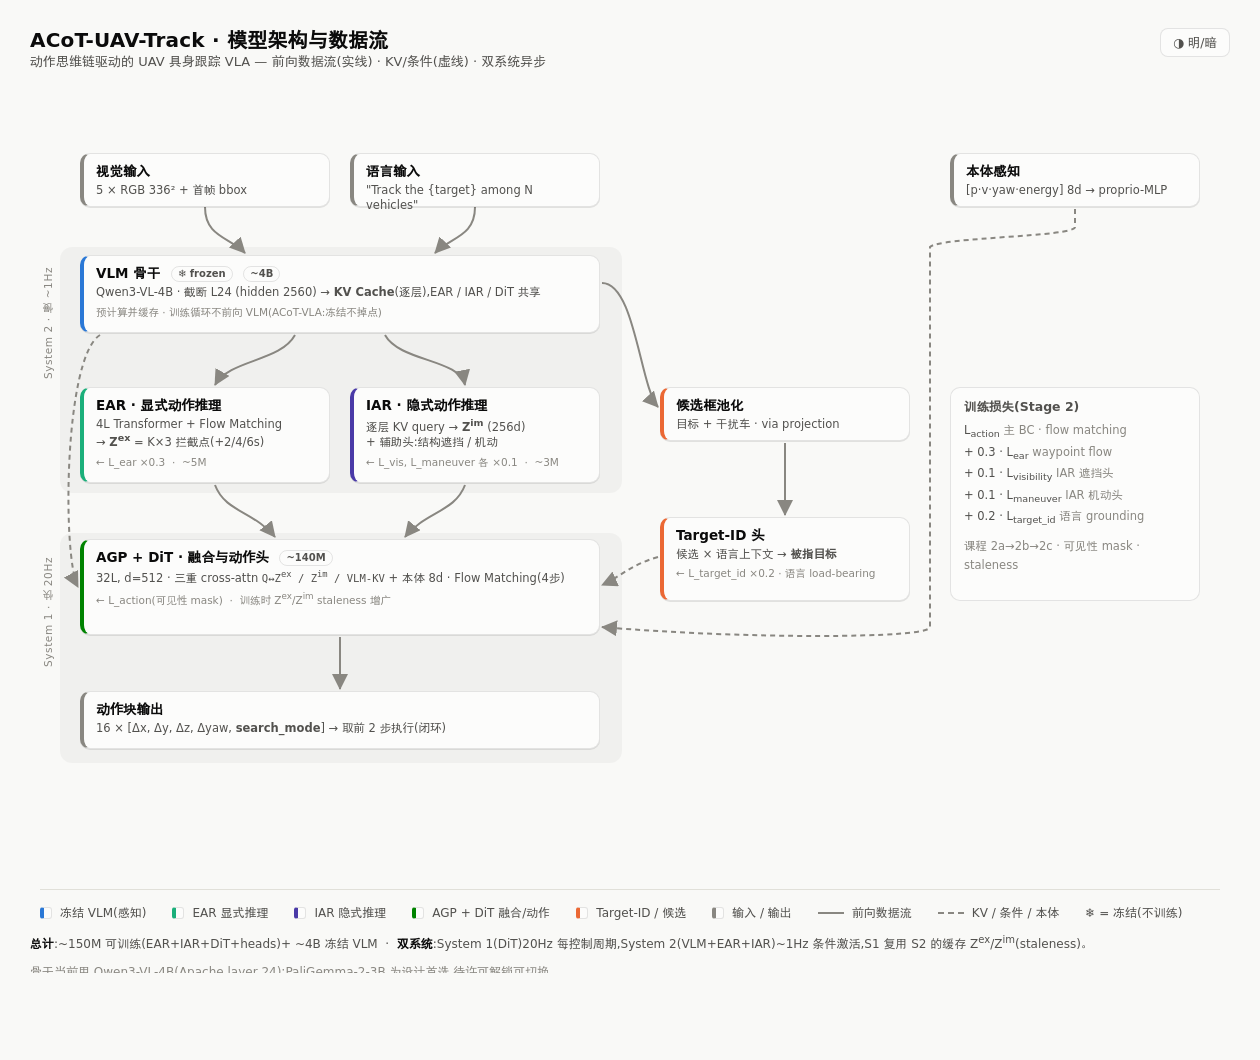
\includegraphics[width=\linewidth]{figures/architecture.png}
\caption{\sys{} architecture and data flow. Solid arrows: forward data
flow. Dashed arrows: KV / conditioning / proprioception. A frozen
vision-language backbone feeds a per-layer KV cache to the Explicit
(\ear{}) and Implicit (\iar{}) Action Reasoners; the Action-Guided
Prediction (\agp{}) head fuses their outputs $\zex,\zim$ with the backbone
KV and proprioception through a flow-matching DiT to emit an action chunk.
System~1 (DiT, 20\,Hz) reuses cached System~2 (\ear{}/\iar{}, $\sim$1\,Hz)
outputs, motivating staleness augmentation at training time
(Section~\ref{sec:training}). \emph{Figure source is the design schematic in
the project notes; a publication vector version is to be produced.}}
\label{fig:arch}
\end{figure}

% Backbone: honest about the probe-gated choice (design doc vs. figure).
\subsection{Frozen vision-language backbone and grounding probe}
\label{sec:method-backbone}
The reasoners read a frozen backbone that is \emph{truncated}: we consume
per-layer KV up to an intermediate layer rather than the final layer. This
imposes a specific constraint---fine-grained grounding must already be
resolved at the truncation layer---that leaderboard-leading final-layer
accuracy does not guarantee. We therefore \emph{select} the backbone by a lightweight
grounding probe run before training: for each candidate we freeze it, read
the truncation-layer features, and train a linear/single-attention read-out
to predict the referred-target box (target vs.\ distractor), passing the
backbone only if grounding is legible at that depth. Under this criterion the
design-preferred backbone is PaliGemma-2-3B (SigLIP${+}$Gemma-2B,
18-layer decoder, truncated near layer~16): its shallow decoder places
grounding early (via a heavy SigLIP encoder and bidirectional prefix
attention) and it shares a lineage with ACoT-VLA and UAV-Track VLA, which
maximises reproducibility of the primary baseline. When grounding requires a
deeper read-out, the current instantiation instead uses Qwen3-VL-4B
(Apache-2.0) truncated near layer~24, as reflected in
Figure~\ref{fig:arch}. The probe doubles as a Stage-0 gate: it quantifies the
frozen backbone's grounding ceiling before any expensive training.
\ph{result: probe target-selection accuracy per backbone $\times$ layer;
final backbone/truncation decision}.

% EAR: three-element pattern (motivation, design, advantage).
\subsection{Explicit Action Reasoner (\ear{})}
\label{sec:method-ear}
\textbf{Motivation.} Predicting where the target will be is a spatial, not a
linguistic, question; expressing it as text and re-decoding into 3D
coordinates introduces a semantic--kinematic gap that is more severe in
6-DoF aerial geometry than on a tabletop.
\textbf{Design.} \ear{} is a four-layer transformer ($d{=}256$, 4 heads,
$\sim$5\,M parameters). Given a noised waypoint sequence and the
backbone KV, self-attention captures temporal dependence among waypoints and
cross-attention injects multimodal context; flow matching denoises noise into
$K{=}3$--$5$ waypoints, each $(x,y,z,\text{confidence})$, projected to
$\zex$. These waypoints are predicted future \emph{target} positions and are
homogeneous with the UAV action space (both are 3D spatial coordinates), so
they guide control without a cross-modal conversion.
\textbf{Advantage over the closest precedent.} TrackVLA++'s Polar-CoT emits
\emph{quantised} 2D polar tokens for a single target point; \ear{} emits a
\emph{continuous} multi-step 3D interception sequence with confidence,
denoised by flow matching, which natively expresses aerial interception
geometry. Because waypoint supervision remains valid through occlusion
(Section~\ref{sec:benchmark-annotation}), \ear{} can point the aircraft at a
target it cannot currently see.

% IAR
\subsection{Implicit Action Reasoner (\iar{})}
\label{sec:method-iar}
\textbf{Motivation.} Some tracking-relevant cues are encoded in the
backbone's intermediate representations but are not expressible as language:
that the target is about to pass behind a building, that it is beginning a
manoeuvre, or that identity-confusion risk is rising as look-alikes appear.
\textbf{Design.} \iar{} ($\sim$3\,M parameters) initialises a learnable
query per backbone layer, down-samples that layer's K/V to a low-dimensional
space, and cross-attends to extract action-relevant features; the per-layer
outputs are average-pooled and projected to a 256-d prior $\zim$. Two
auxiliary heads---structural-occlusion prediction and manoeuvre
detection---shape $\zim$ during training.
\textbf{Advantage.} This inherits ACoT-VLA's per-layer KV query mechanism;
our adaptation is the aerial cue set above and the use of the separated
\texttt{occ\_structural} signal (not the merged occlusion signal) to train
the occlusion head, so ``about-to-be-occluded'' is learned rather than
``already off-screen''.

% AGP + search_mode
\subsection{Action-Guided Prediction head and continuous \texttt{search\_mode}}
\label{sec:method-agp}
\textbf{Design.} The \agp{} head is a 32-layer DiT ($d{=}512$, 8 heads,
$\sim$140\,M parameters). An action query cross-attends in interleaved
fashion to $\zex$ (coarse waypoint guidance), $\zim$ (implicit prior), and the
backbone KV (global semantic context), while proprioception is embedded by an
MLP; flow matching (4 denoising steps) emits a $16$-step action chunk, of
which the first two steps are executed before the next System-1 cycle.
\textbf{Continuous search.} The last action dimension,
$\texttt{search\_mode}\in[0,1]$, replaces discrete track/search/recover
switching with a single value that grows from precise tracking, through
widened field-of-view and predicted-trajectory search, to full-area scan.
\textbf{Honest note on supervision.} \texttt{search\_mode} is
\emph{explicitly supervised} by the hand-crafted label of
Section~\ref{sec:benchmark-annotation} (an MSE visibility loss); it is a
differentiable regression target, \emph{not} an emergent signal. Its
advantage over discrete switching is being continuous and threshold-free
(avoiding chattering / Zeno-style spurious mode flips), not spontaneity. An
emergence claim would require removing the explicit supervision and is left
to future work.

% =====================================================================
\section{Training Strategy}
\label{sec:training}

Three architectural constraints---a frozen truncated backbone, a privileged
expert, and asynchronous two-system inference---determine the training
recipe. The backbone is frozen and its truncated KV/features are
\emph{precomputed and cached} once over the dataset, so the training loop
never runs the backbone forward; ACoT-VLA reports no accuracy loss from
freezing, and with only $\sim$150\,M trainable parameters this permits
large batches on a single GPU.

\paragraph{Staged pipeline.}
\emph{Stage 0 (optional warm-start).} Grounding is warmed from aerial
language-localisation data and the flight-action distribution from an
open-source pedestrian-domain drone corpus; the domain gap (pedestrian
$\to$ vehicle, passive $\to$ active) means this is initialisation only.
\emph{Stage 1 (\ear{} warm-up).} With the backbone, \iar{}, and DiT frozen,
\ear{} is trained on clean waypoint ground truth
($L_{\mathrm{flow}} + \lambda\,L_{\mathrm{temporal}}$). Gate: waypoint MSE
$<\!10\,\mathrm{m}$ @ $6\,\mathrm{s}$, \emph{and} the predicted trajectory belongs to
the target rather than a distractor---an early language-grounding check
without which everything downstream is void.
\emph{Stage 2 (end-to-end curriculum).} With the backbone frozen, \ear{},
\iar{}, DiT, \agp{}, and the proprioception MLP are trained jointly under
\[
L = L_{\mathrm{action}} + 0.3\,L_{\mathrm{ear}}
    + 0.1\,(L_{\mathrm{visibility}} + L_{\mathrm{maneuver}})
    + 0.2\,L_{\mathrm{target\text{-}id}},
\]
where $L_{\mathrm{target\text{-}id}}$ classifies which candidate box is the
referent, routing language directly into the gradient as the training-side
support for load-bearing language. Two design elements are essential.
\emph{Curriculum} (single target $\to$ easily-distinguished distractors
$\to$ visually similar distractors with counterfactual language) prevents
the ``follow the centre'' shortcut from being learned first.
\emph{Staleness augmentation} randomly reuses stale \ear{}/\iar{} outputs so
that training matches the up-to-20-frame-old cache that System~1 reads
at inference. The action-imitation loss is masked on \texttt{occluded}
frames (the expert used privileged truth the student cannot see), while
waypoint loss is \emph{not} masked, so the model keeps learning where the
target will reappear.
\emph{Stage 3 (optional closed-loop RL).} With the backbone, \ear{}, and
\iar{} frozen, the last DiT layers (or LoRA) are refined by GRPO on CARLA
on-policy rollouts to treat the three ailments of behaviour cloning
(compounding error, sub-optimal occlusion recovery, no exploration). The
reward must include an identity term $R_{\mathrm{correct\text{-}id}}$;
without it, RL degenerates into ``follow any car'' to farm the tracking
reward and unlearns disambiguation.

\paragraph{Validation gates and splits.}
Gates are embedded in the pipeline, not deferred: a triple held-out (town,
vehicle model, distractor-count configuration) guards against
limited-map memorisation, and each stage runs a reduced evaluation that must
pass before the next begins (waypoint attribution at Stage~1; mis-follow,
w/o-language ablation, and counterfactual-language switching at Stage~2;
success/recovery and a reward-hacking check at Stage~3).

% =====================================================================
\section{Experiments}
\label{sec:experiments}

\emph{Status: the model is being trained; this section specifies the
protocol and reports placeholders. Every \ph{\dots} is a value to be
measured, not a claim.}

\subsection{Protocol}
\label{sec:exp-protocol}
We evaluate on held-out episodes of the benchmark
(Section~\ref{sec:benchmark}), stratified by disambiguation strategy and
target class, with a held-out town for a coarse cross-map check (the MVP has
few maps; strong generalisation is deferred to the scaled release).
Optimisation for Stage~2 follows the notes: AdamW, learning rate
$10^{-4}$, batch size \chk{64}, on \chk{4$\times$A40 (48\,GB)} \ph{confirm
final hardware / batch}.

\subsection{Baselines}
\label{sec:exp-baselines}
Table~\ref{tab:baselines} lists the comparison set. UAV-Track VLA is the
primary competitor; the appearance/motion-only (no-language) baseline is the
key control for the load-bearing-language claim. We include a self-built
Language-CoT head (ECoT-style, text$\to$box$\to$3D) to isolate action-space
versus language-space reasoning, and ablations that remove \ear{}, \iar{},
and language. TrackVLA++ is ground/human and enters as a discussed precedent;
if run as a baseline, its ground-to-air adaptation limits must be stated. We
do not include the non-existent ``CosFly-VLA'' referenced in early notes;
it is not a real system.

\begin{table}[t]
\centering
\caption{Comparison set and what each entry tests. ``Ours'' rows are the
full model and its ablations.}
\label{tab:baselines}
\small
\begin{tabular}{@{}lll@{}}
\toprule
Method & Type & Tests \\
\midrule
\sys{} (ours) & full model & --- \\
UAV-Track VLA \citep{uavtrackvla} & published, primary & aerial language tracking; diff.\ = disambiguation \\
DeTrack \citep{detrack} & published & UAV closed-loop, moving distractors, no language \\
$\pi_{0.5}$ fine-tuned \citep{pizerohalf} & generic VLA & no UAV specialisation, no reasoning \\
Language-CoT head (ours) & reasoning control & action-CoT vs.\ language-CoT (H3) \\
Appearance/motion-only (ours) & \textbf{key control} & is language load-bearing? \\
\sys{} w/o \ear{} & ablation & explicit-reasoning contribution (H1) \\
\sys{} w/o \iar{} & ablation & implicit-prior contribution (H2) \\
\sys{} w/o language & ablation & language contribution (\S\ref{sec:lang-necessity}) \\
\bottomrule
\end{tabular}
\end{table}

\subsection{Metrics}
\label{sec:exp-metrics}
Success Rate (target kept in view to episode end); \textbf{Mis-follow Rate /
ID-correctness} (fraction of episodes tracking the wrong vehicle---the direct
measure of disambiguation and the core evidence for language); Occlusion
Recovery Rate (re-lock within $N$ seconds); Average Tracking Frames; Search
Mode Efficiency (time fraction with $\texttt{search\_mode}{>}0.5$, lower is
better); and Cross-town SR drop (seen$\to$unseen CARLA map, \emph{in-sim
generalisation only}, not real flight). Following ACoT-VLA's observation that
saturated success rates hide the real story, we lead with robustness
metrics---occlusion recovery, mis-follow, continuous tracking length---rather
than clean-scene success rate.

\subsection{Main comparison}
\label{sec:exp-main}
\ph{result: Table of SR $\uparrow$ / Mis-follow $\downarrow$ / Occlusion
Recovery $\uparrow$ / Avg Tracking Frames $\uparrow$ for all methods in
Table~\ref{tab:baselines}}. Expected reading:
\sys{} matches or exceeds UAV-Track VLA on success while substantially
lowering mis-follow rate, with its largest margin over the appearance-only
control. Table~\ref{tab:main} is the empty shell to be filled.

\begin{table}[t]
\centering
\caption{Main results on the held-out benchmark split. \textbf{All cells are
placeholders} pending training. Arrows give metric direction.}
\label{tab:main}
\small
\begin{tabular}{@{}lcccc@{}}
\toprule
Method & SR $\uparrow$ & Mis-follow $\downarrow$ & Occ.\ Rec.\ $\uparrow$ & Avg.\ Frames $\uparrow$ \\
\midrule
$\pi_{0.5}$ fine-tuned & \ph{--} & \ph{--} & \ph{--} & \ph{--} \\
UAV-Track VLA & \ph{--} & \ph{--} & \ph{--} & \ph{--} \\
Appearance/motion-only & \ph{--} & \ph{--} & \ph{--} & \ph{--} \\
Language-CoT head & \ph{--} & \ph{--} & \ph{--} & \ph{--} \\
\sys{} (ours) & \ph{--} & \ph{--} & \ph{--} & \ph{--} \\
\bottomrule
\end{tabular}
\end{table}

\subsection{Hypotheses and ablations}
\label{sec:exp-ablation}
The experiments test three hypotheses, each tied to a design element:
\textbf{H1}, explicit waypoint prediction beats purely implicit backbone
features (\sys{} vs.\ w/o \ear{}; largest gap expected in occlusion
recovery); \textbf{H2}, the implicit prior contributes independently under
occlusion/manoeuvre (\sys{} vs.\ w/o \iar{}; expected at sharp turns/stops);
\textbf{H3}, action-space reasoning beats language-space reasoning (\sys{}
vs.\ Language-CoT head; expected because 3D waypoints avoid the 2D-box$\to$3D
conversion). \ph{result: ablation table with $\Delta$ to full model for
w/o-\ear{}, w/o-\iar{}, w/o-language, and Language-CoT}.

\subsection{Language-necessity verification}
\label{sec:lang-necessity}
This is the experiment on which the core claim stands or falls. We run four
checks. (1) \emph{Appearance/motion-only baseline}: if its mis-follow rate is
already low, language is unnecessary and the task must be made harder. (2)
\emph{w/o-language ablation}: the rise in mis-follow rate when language is
removed from the full model is the net contribution of language. (3)
\emph{Counterfactual language}: on a fixed frame, re-pointing the sentence at
a different vehicle should switch which vehicle the agent follows---the
strongest evidence that the model reads language. (4) \emph{Expert-ceiling
statement}: imitation of a P-only PID is bounded by that PID, so any claim of
exceeding it requires the Stage-3 RL result, and otherwise the model's value
is framed as disambiguation and recovery, not tracking precision.
\ph{result: mis-follow rate for appearance-only vs.\ full vs.\ w/o-language;
counterfactual-language switch success rate}. The pre-registered pass
condition is that removing language significantly raises mis-follow rate and
that counterfactual re-pointing switches the target; if not, the task is too
easy and is hardened before any headline claim is made.

% =====================================================================
\section{Discussion and Limitations}
\label{sec:discussion}

We state boundaries directly, since several are reviewer-critical.

\paragraph{Contribution boundary.}
The reasoning mechanism (EAR/IAR/AGP action-space chain-of-thought) is
transferred from ACoT-VLA \citep{acotvla}, and action-space reasoning for
tracking has a ground precedent in TrackVLA++ \citep{trackvlapp}; we do not
claim either as novel. The defensible contribution is the task/benchmark
intersection---active aerial flight $+$ language-specified vehicle $+$
visually-similar-vehicle disambiguation $+$ closed-loop control---and its
adaptation and evaluation, positioned honestly as an application/benchmark
contribution rather than a new architecture.

\paragraph{Simulation and domain gap.}
Evaluation is CARLA-only. Aerial assets are designed for street-level views
so top-down fidelity is weaker, agent motion is scripted, and there is no
real multirotor dynamics; all aerial competitors we compare against are
likewise sim-only. Sim-to-real transfer is unaddressed here and is the single
strongest missing piece; a small real-flight demonstration of
language-specified, distractor-robust tracking would be the most decisive
differentiator and is future work.

\paragraph{Data-scale limits.}
The MVP release ($\sim$100K frames, few maps) is sufficient for convergence
and preliminary ablations but not for statistically-strong ablations, strong
cross-map generalisation, or SOTA-scale comparison; similar-distractor
co-visibility (13.6\%) and structural occlusion
(4.3\%) are lower than ideal for the strongest occlusion (H2)
evidence. The planned publication-scale regeneration ($\sim$300K frames,
more maps, redesigned occlusion scenes) is required before the full claims
are made, and episode-level scale (target: several thousand episodes, versus
DeTrack's $11{,}368$ trajectories) is the axis on which the benchmark should
be reported, not frame count alone.

\paragraph{Expert ceiling and failure modes.}
Because the expert is a privileged P-only PID, behaviour cloning cannot
exceed its control precision; the model's intended value is disambiguation
and occlusion recovery. We expect failure modes to include latching onto a
similar distractor during long co-visibility, drift during extended
occlusion beyond the waypoint horizon, and RL reward-hacking toward
``nearest car'' if $R_{\mathrm{correct\text{-}id}}$ is under-weighted;
Section~\ref{sec:experiments} is designed to surface these rather than hide
them.

% =====================================================================
\section{Conclusion}
\label{sec:conclusion}

We introduced \sys{}, a vision-language-action model and CARLA benchmark for
language-conditioned aerial embodied tracking with similar-distractor
disambiguation---an intersection of active flight, a language-specified
vehicle target, visual disambiguation among look-alike vehicles, and
closed-loop control that, to our knowledge, no prior system addresses in
full. The model transfers ACoT-VLA's action-space chain-of-thought (explicit
3D-waypoint reasoning, implicit backbone priors, a fused flow-matching action
expert) into 6-DoF aerial interception geometry and replaces discrete
track/search switching with a continuous, differentiable search dimension;
the benchmark's scene design and counterfactual-language protocol are built
to keep language load-bearing, and the evaluation is organised around
mis-follow rate, occlusion recovery, and language-necessity ablations.
Because model training is still in progress, the empirical claims in this
draft are placeholders; completing Stage-1 and Stage-2 training and filling
the language-necessity results is the immediate next step, followed by
publication-scale data regeneration and, ideally, a real-flight
demonstration.

% =====================================================================
\section*{Reproducibility and honesty statement}
The benchmark, data-generation pipeline, annotation projection (verified
$\Delta u{=}\Delta v{=}0$ against the CARLA runtime), and evaluation code
will be released. This draft deliberately marks all unmeasured quantities as
placeholders and all not-yet-verified citations for author checking; no
experimental result reported here should be read as measured until its
placeholder is replaced.

% =====================================================================
\bibliographystyle{plainnat}
\bibliography{references}

\end{document}
